% !TeX root = ../main.tex
\cleardoublepage
\chapter{引言}\label{ch:bg}



\section{课题背景}\label{sec:bg-bg}


\subsection{IC装备}\label{sec:bg-bg-ic}

IC产业是一个国家现代工业的基础,是信息产业的核心,因此发展具有战略意义的集成电路产业以占领科技、经济和军事制高点已经成为许多国家的共识。工信部发布的《集成电路产业“十二五”发展规划》中提出,到“十二五”末,集成电路产量超过1500亿块,销售收入达3300亿元,年均增长18\%,占世界集成电路市场份额15\%左右,满足国内近30\%的市场需求。IC制造需要大量高技术制造装备;整个IC产业的迅速发展,也带动了IC装备制造业的发展。其中,关键制造装备的国产化是大势所趋。IC制造工艺可分为四大类:沉积(deposition),去除(removal),布线(patterning),改性(modification of electrical properties),其中最常见的工艺包括PVD/CVD(物理/化学气相沉积)、等离子体刻蚀、化学机械平整化、旋转涂覆、光刻、离子移植、快速退火等。从单晶硅制成的晶圆,到最后的成品芯片,要依次经历多达300道工序。所有的IC工艺均需在严格受控的条件下进行,这需要大量专用设备的支持。


\subsection{静电卡盘简介}\label{sec:bg-bg-chuck}

卡盘(chuck)是IC装备中重要的通用组件,用于夹取、搬运、或固定晶圆(wafer)及其他薄片类工件(如光刻掩模等)。依据其夹紧原理,主要可分为机械卡盘、真空吸盘和静电卡盘三种。机械卡盘需与工件保持紧固的机械接触,适用于要求不高或需要传动的场合,如搬运、旋转涂覆等;真空吸盘必须工作在大气环境下,与工件接触力极小,最适合用于搬运;静电卡盘结构、原理均复杂,但吸附力均匀稳定,且能满足各类工艺所需的额外要求,广泛用于工艺装备中。

\subsubsection{静电卡盘组成}\label{sec:bg-bg-chuck-component}

图~\ref{fig:bg-echuck-sch}~为一典型静电卡盘及其配套系统的简化示意图。其中,与本文直接相关的主要组成部分如下:

\begin{enumerate}
  \item \textbf{静电电极与高压静电电源}:
    静电卡盘核心元件,用于产生静电吸附力。静电电极通常为极薄的一层金属,其材料为\ce{Mo}、\ce{Al}等。静电电源可产生高达数千伏的静电电压。
  \item \textbf{陶瓷介电层}:
    静电卡盘核心元件,在静电电极与被吸附的工件之间起到绝缘作用。陶瓷介电层具有较高的电阻率以及抗击穿电压,且其接触工件的表面平面度与光洁度要求均较高。根据静电卡盘原理不同,陶瓷层材料也不同,通常采用\ce{Al2O3}、\ce{AlN}、\ce{SiO2}等。
  \item \textbf{气体界面层与背吹通道}:
    气体界面层处于陶瓷介电层与工件之间,其厚度为\si{\um}量级,一般采用导热性强、活性差的气体,如\ce{He}、\ce{Ne}等,主要用于冷却工件,控制其背面温度均匀分布且不超过规定的上限。这层气体由外部气源通过静电卡盘内部的背吹分配板以及陶瓷介电层中的背吹通道输送到工件与介电层之间产生。
  %TODO:finish component list
\end{enumerate}

\begin{figure}[tb]
\centering
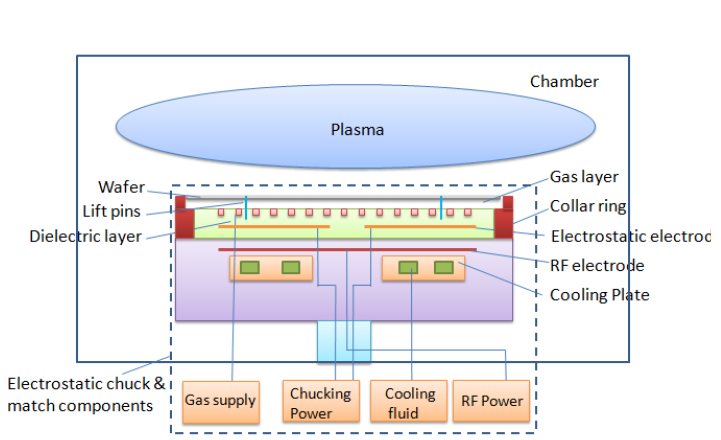
\includegraphics[width=0.8\linewidth]{bg/echuck__sch.png}
\caption{静电卡盘组成示意图}
\label{fig:bg-echuck-sch}
\end{figure}

\subsubsection{静电卡盘工作原理}\label{sec:bg-bg-chuck-principle}

静电卡盘的基本工作原理是在工件与卡盘间产生一强静电场,通过感应在工件表面产生表面电荷,进而产生静电吸引力,将工件吸附在静电卡盘的介电层表面。由于静电力为场力,静电卡盘产生的吸附力均匀、稳定。并且,在吸附工件的基础上,静电卡盘还起到控制工件表面温度及均匀性、抑制工件热形变、控制工艺腔室中等离子体能量与溅射方向(刻蚀应用)、保证工件平面度(光刻应用)等作用。

根据静电力产生的基本机理,可将静电卡盘分为两大类:库仑型、\mbox{J-R} (Johnson-Rahbek)型。 以下对比二者的主要特点与差异:

库仑型的介电层电阻率较高($\rho > \SI{1e14}{\ohm\cm}$),基本可认为是绝缘体,工作原理类似平行板电容器,如图~\ref{eq:bg-coulomb}。其产生的静电力 较小,但较稳定、均匀,且残余电荷影响较小。静电力理论公式为:
\begin{equation}
\label{eq:bg-coulomb}
F = \frac{1}{2} {\varepsilon}_0 \, A \, {\left( \frac{k_{\mathrm{d}} U}{d} \right)}^2
\end{equation}

\begin{figure}[h]
\centering
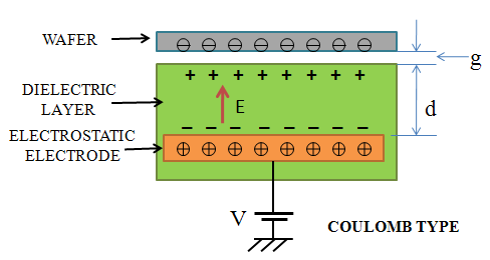
\includegraphics[width=0.70\linewidth]{bg/echuck__sch__coulomb.png}
\caption{库仑型静电卡盘原理示意图}
\label{fig:bg-echuck-sch-coulomb}
\end{figure}

\mbox{J-R}型的介电层为半导体,电阻率较低($\rho = \SIrange{1e10}{1e12}{\ohm\cm}$),工作原理依赖流过介电层的电流以及介电层与工件之间的接触电阻,如图~\ref{eq:bg-jr}。其产生的静电力较大,但不稳定,且受残余电荷影响严重。静电力理论公式为:
\begin{equation}
\label{eq:bg-jr}
F = \frac{1}{2} {\varepsilon}_0 \, k_{\mathrm{g}} \, A_{\mathrm{eff}} \, {\left( \frac{U_{\mathrm{eff}}}{g} \right)}^2
\end{equation}

\begin{figure}[h]
\centering
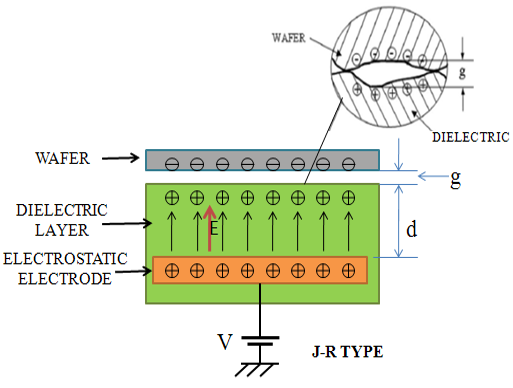
\includegraphics[width=0.70\linewidth]{bg/echuck__sch__jr.png}
\caption{\mbox{J-R}型静电卡盘原理示意图}
\label{fig:bg-echuck-sch-jr}
\end{figure}

本文中主要讨论静电力较为稳定的库仑型静电卡盘的特性。

\subsubsection{静电卡盘主要性能指标}\label{sec:bg-bg-chuck-spec}

在设计静电卡盘时,需评价其性能指标优劣。静电卡盘主要的性能指标及其意义如下:

\begin{enumerate}
  \item \textbf{静电吸引力大小}:
    静电卡盘核心参数,设计时希望在尽可能低的电压下获得尽可能高、稳定、均匀的静电力。与静电力大小直接相关的性能指标包括击穿电压、静态电流等。
  \item \textbf{残余电荷与残余力大小}:
    当去除静电卡盘电极电压时,感生出的电荷并未马上消失,留在介电层与工件表面的残余电荷会产生残余静电力,使得工件不能马上从卡盘上移除,影响生产效率。设计时希望能尽量减小残余静电力大小以及残余电荷衰减时间。
  \item \textbf{工件表面温度及其均匀性}:
    沉积、刻蚀等工艺对工件表面温度较敏感,若工件表面温度超过规定值或不均匀,则会影响工艺结果。需由静电卡盘的冷却与背吹系统保证工件表面温度均匀且在规定值内。
  %TODO:finish spec list
\end{enumerate}

其中,静电吸引力大小是最主要的性能指标,这是因为静电吸引力是静电卡盘的基本功能,其他性能指标(如温度分布、平面度等)均直接或间接受其大小影响,且强静电场是整个多场耦合系统中的重要的组成部分。因此,有必要研究静电吸引力的产生机理、影响其大小的因素、以及检测其大小的有效手段。



\section{国内外研究现状}\label{sec:bg-prior}

国内针对静电吸引力的相关研究极其缺乏,在各文献数据库中均未搜索到相关成果。其他静电卡盘相关的成果多为企业专利等,多用于保护其独创设计。相比之下,国外对静电吸引力有一定数量的研究,主要集中于其产生机理、等效模型、理论与经验公式、定性与定量实验验证等方面。然而多数针对静电力大小的研究中,即使有定量实测静电力,往往采用的方法较为简单,且未加以详细描述或有对检测方法的深入研究。以下简要介绍各文献中提及的静电力检测方法。


\subsection{机械提拉法}\label{sec:bg-prior--pull}

该类方法在文献中较为常见,如日本日立高科、山形大学、韩国延世大学、荷兰TNO TPD等单位的研究中均使用该类方法检测静电力大小。其原理简单而直接,如图~:使用直线电机、电动推杆或气缸等作为执行器,通过连接件向已吸附的晶圆施加一个向上(远离静电卡盘表面)的拉力;当该力逐渐增大,与静电力相平衡时,即发生脱附现象;通过力传感器记录此拉力即可得到静电力大小。

\begin{figure}[tbh]
\centering
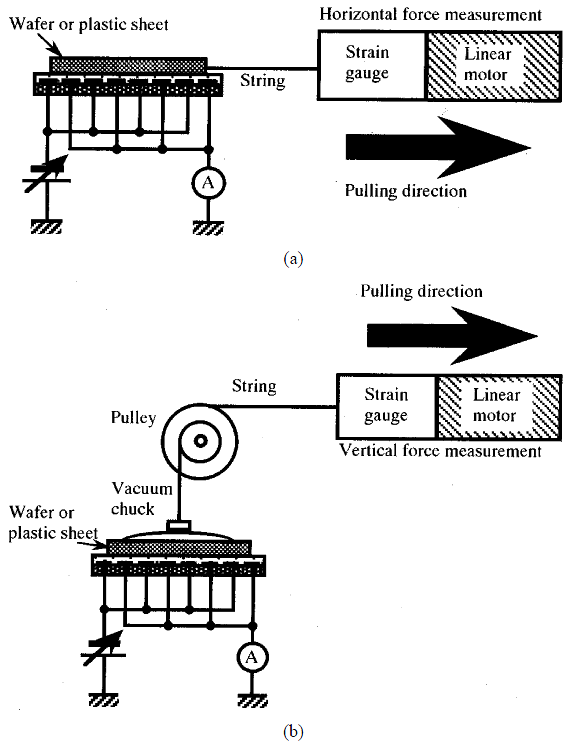
\includegraphics[max size={0.618\linewidth}{0.66\textheight}]{bg/prior__pull.png}
\caption{机械提拉法原理示意图}
\label{fig:bg-prior-pull}
\end{figure}


\subsection{背吹平衡法}\label{sec:bg-prior-pressure}

机械提拉法的一个主要问题是难以保证提拉时晶圆均匀受力,导致静电力受部分脱附影响很大。在文献中出现较多的另一种检测思路是背吹平衡法,可一定程度上解决此问题。该方法较为典型的应用 是在日本名古屋大学、中国台湾大学的研究中、以及中国北方微电子公司的实际试验中,其主要原理如下:利用静电卡盘的背吹通道创造一个压强受控的气体界面层,当气体在被吸附的晶圆背面产生的压强与静电力相平衡时,即发生脱附现象;可通过多种方式检测脱附现象,并通过压强推算出静电力大小。由于气体压力是分布力,背吹平衡法可保证晶圆受力均匀性。具体的原理分析见第\ref{ch:principle}章中相关讨论。


\subsection{形变检测法}\label{sec:bg-prior-warp}

已有静电力检测方法中,只有形变检测法能够定性测出静电力分布情况。该方法于美国University of Wisconsin-Madison与德国Fraunhofer Institut für Angewandte Optik und Feinmechanik的合作研究、以及德国Berliner Glas KGaA的研究中分别独立提出。其主要检测原理如下:特别制作一个晶圆,其一面具有凸台阵列特征,将这一面朝向静电卡盘,加电吸附后,使用激光干涉仪获得晶圆各处的挠度(即宏观形变,如图~\ref{fig:bg-prior-warp}),并与仿真结果对照,即可定性判断出静电力相对大小以及分布情况。

\begin{figure}[tbh]
\centering
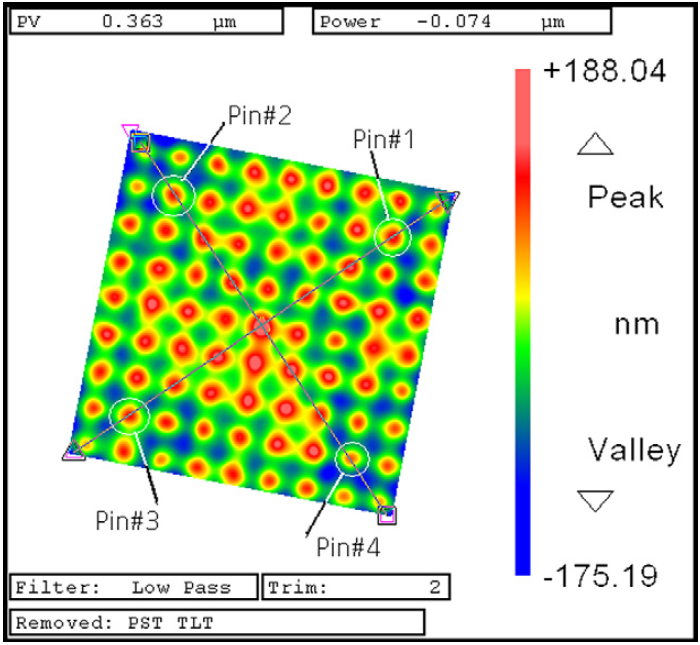
\includegraphics[width=0.618\linewidth]{bg/prior__warp.png}
\caption{形变检测法原理示意图}
\label{fig:bg-prior-warp}
\end{figure}



\section{问题的提出}\label{sec:bg-problem}

由\ref{sec:bg-bg-chuck-spec}节讨论,静电力大小是静电卡盘最主要的性能指标之一,也是设计优化的重要目标之一,但其产生、消除机理复杂,目前尚无十分精确的模型,因此需要通过实验方法来检测静电力的大小。已有的静电力检测方法中仍具有很多不足之处,如:有些检测方法只适合于定性判定静电力相对大小,不能准确求得其具体数值;多数检测方法需判定晶圆完全脱附,但晶圆脱附往往为一连续过程,导致判定失效或引入系统误差;另外,晶圆脱附时,晶圆与卡盘的间隙已改变,而由\ref{sec:bg-bg-chuck-principle}节知,静电力大小也随之发生改变,为了减小检测中的系统误差,应减小或消除检测系统对被检测对象产生的干扰。

基于以上分析,本文将以已有检测方法中最为可靠的背吹平衡法为基础,通过对其具体原理的分析,找出其中影响检测准确性的因素,并加以改进,设计出改进的检测方案(第\ref{ch:principle}章);然后以此为基础,设计完整的静电力检测平台(第\ref{ch:rig}章),并将其实际搭建出来(第\ref{ch:impl}章);最后通过在其上开展静电力检测试验(第\ref{ch:exp}章),分析试验结果(第\ref{ch:analysis}章),验证本文设计的改进方案以及检测平台可以更准确地检测静电力大小。